\chapter{Node - Express Webanwendung}
\label{sec:nodechapter}
\lhead{Kapitel 6. \emph{Node - Express Webanwendung}}

\section{Allgemein}
\label{sec:nodechapter-general}
Wir als Studenten haben durch das Studium, aber auch durch Nebenjobs und private Projekte Erfahrungen
mit verschiedenen Programmierkonzepten sammeln können. Da wir bei der Entwicklung der Pepper Anwendung
jedoch nur zwischen den Sprachen Kotlin und Java entscheiden konnten, haben wir zu Beginn unseres Projektes,
das Gefühl gehabt, in unserer Entwicklung, was die Nutzung und Implementierung verschiedener
Methoden angeht, sehr eingeschränkt zu sein.

Daher haben wir im Verlauf unseres Bachelorprojektes immer wieder gemerkt, dass mit dem Pepper allein nicht viel anzufangen
ist, wenn es um Flexibilität in der Entwicklung geht. Zugriff auf Berührungssensoren, sowie die Kamera und die Mikrophone
sind nicht direkt möglich, sondern nur über vordefinierte Funktionen der Aldebaran Bibliotheken. Somit haben
wir keine Möglichkeit, selbst Gesichter zu erkennen oder Sprache zu analysieren, geschweige denn mehr als nur mit Pepper
reden zu können.

\begin{figure}[H]
    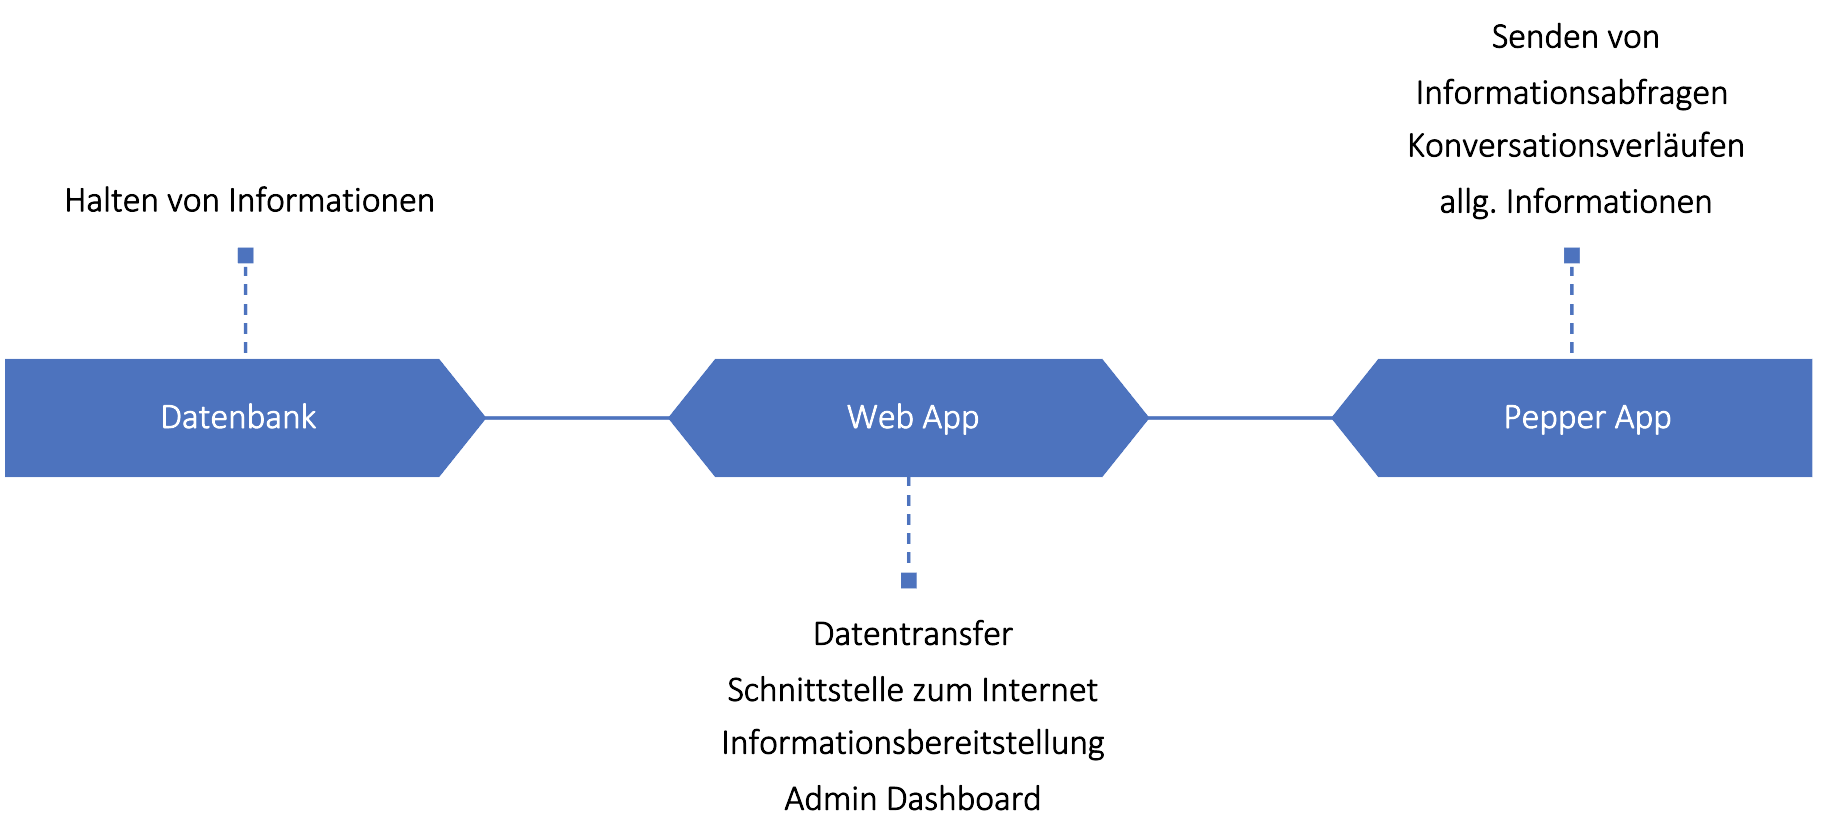
\includegraphics[width=\textwidth]{Figures/NodeChapter/integration.png}
    \caption{Zusammenhang: Pepper App und Backend}
    \label{fig:integration}
    \centering
\end{figure}

Bei der Implementierung der Stundenpläne etwa, werden verschiedene Anfragen an die Hochschulserver geschickt und ausgewertet,
jedoch ist auch dies in Java nicht wirklich entwicklerfreundlich. Daher sind wir auf die Idee gekommen,
einen Webserver aufzusetzen, den Pepper kontaktieren kann, um weiterführende Informationen zu erhalten.

Genau hier war es uns von Vorteil, schon Erfahrungen mit Node, Datenbanken und API's gesammelt zu haben.
Daher ist es ein leichtes Unterfangen gewesen, einen Express Webserver mit Hilfe der Laufzeitumgebung Node aufzusetzen,
auf welchem wir vielfältige Möglichkeiten zur Implementierung von komplexen Vorgängen haben.

So hat es sich ergeben, dass wir nicht nur eine Anwendung für Pepper entwickeln wollen, sondern einen
zweiten Schwerpunkt festlegen, welcher sich auf das Sammeln und Auswerten von Daten konzentriert. Diese Daten
sollen natürlich von Pepper über unsere Anwendung gesammelt werden.

Das Repository dieser Webanwendung ist öffentlich und unter folgender Adresse erreichbar:

\href{https://github.com/ProjectPepperHSB/NodeJS\_Server4Pepper}{https://github.com/ProjectPepperHSB/NodeJS\_Server4Pepper}

\section{Überblick: Webanwendung}
\label{sec:nodechapter-ueberblick}
\lhead{Kapitel 6. \emph{Node - Express Webanwendung: Überblick}}
Bevor wir im Folgenden auf die Implementierung und Spezifikationen unserer Webanwendung eingehen, wollen wir hier kurz
die Hauptfunktionalitäten, welche wir in drei Kategorien aufgeteilt haben, aufzeigen.

\begin{figure}[H]
    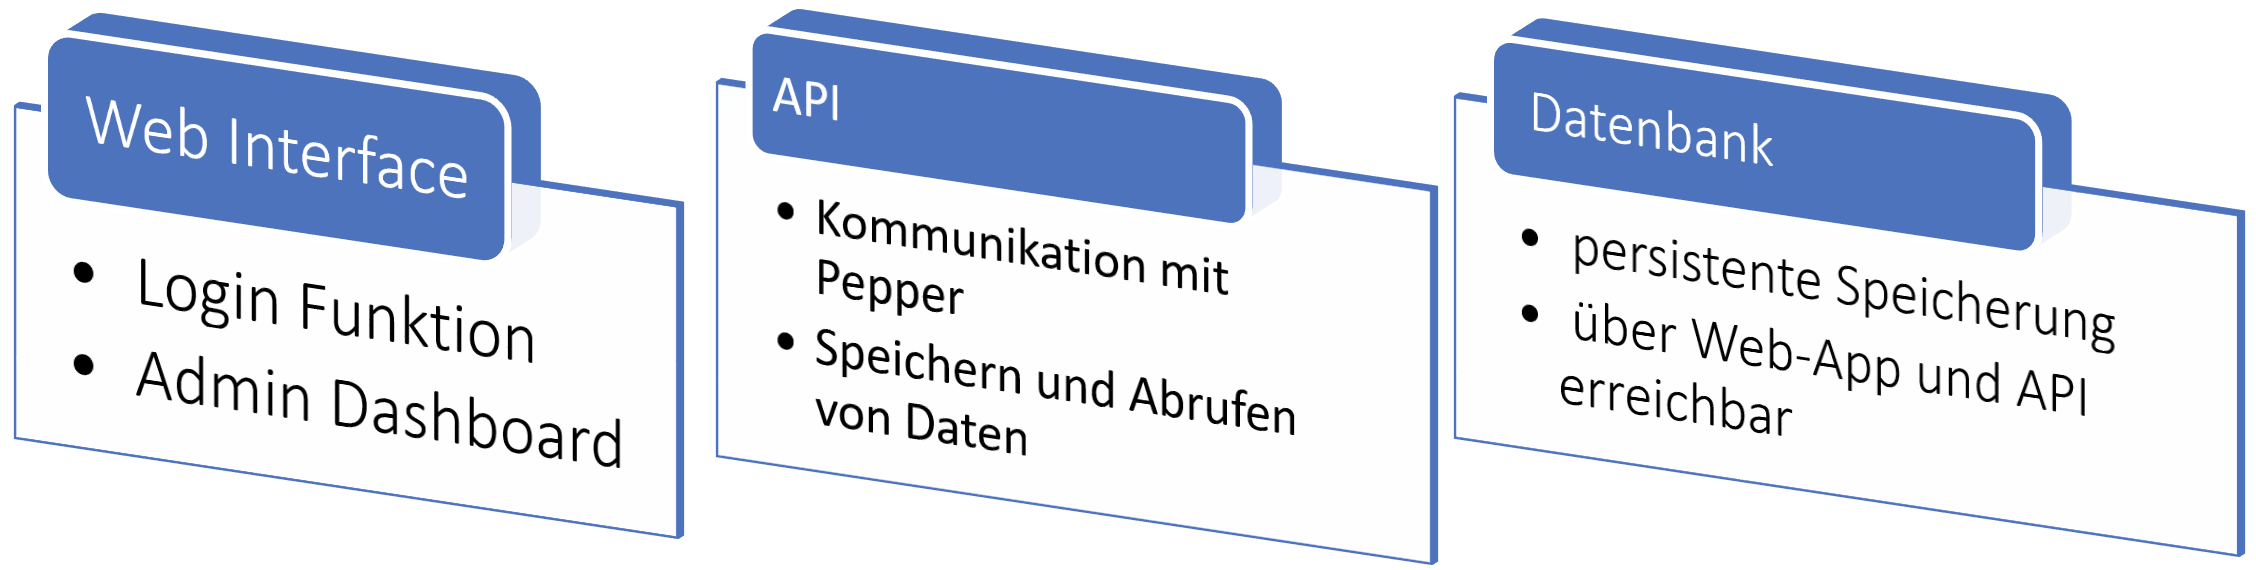
\includegraphics[width=\textwidth]{Figures/NodeChapter/WebAppComponents.png}
    \caption{Komponenten der Webanwendung}
    \label{fig:webappcomponents}
    \centering
\end{figure}

Diese Webanwendung, sowie die dazugehörige Datebank laufen derzeit auf dem Hochschulserver Hopper in einem
abgeschirmten Docker Kontainer, welcher einem Benutzer mit Namen ``hbv-kms'' gehört. Dies ist ein
Benutzer, auf welchen wir gemeinsam als Team zugreifen können. Da die Anwendung über den HTTP
Port des Dockers läuft, findet sich der Pfad ``docker-hbv-kms-http'' in allen Endpunkten dieser Webanwendung wieder.

Sie ist jedoch auch auf fast jedem lokalen Rechner ausführbar, sofern eine funktionsfähige MySQL Instanz aktiv ist.
(vgl. Abschnitt \ref{sec:nodechapter-implementation})

\subsection{Web Interface}
\label{sec:nodechapter-web-interface}
Das Web Interface dient dazu, den Entwicklern und Betreibern der Webanwendung Informationen über die gesammelten Daten
aufzuzeigen. Da wir es für sinnvoll halten, nicht jedem den kompletten Zugriff auf die gesammelten Daten zu gewähren, haben
wir uns dazu entschieden, nur einen Benutzer in unserer Webanwendung anzulegen, welcher Zugriff auf das Admin Dashboard hat.
Somit sparen wir uns die Implementierungen zur Registration und Verwaltung von Nutzern.
(weiteres in Abschnitt \ref{sec:nodechapter-implementation}.\\


\begin{figure}[H]
    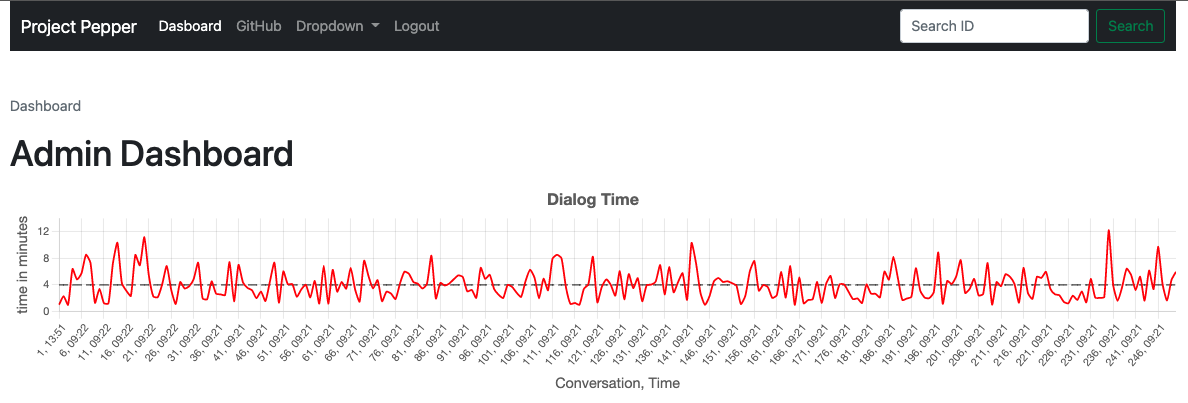
\includegraphics[width=\textwidth]{Figures/NodeChapter/adminDashboard1.png}
    \caption{Webansicht des Admin Dashboards Teil 1}
    \label{fig:admindashboard1}
    \centering
\end{figure}

(Abb. \ref{fig:admindashboard1}) Sofern sich ein Administrator angemeldet hat, gelangt er in die Ansicht des Admin Dashboards.
Dieses besteht aus mehreren Komponenten. Zu sehen ist, dass sich am oberen Bereich der Abbildung eine Menüleiste befindet.
Diese Beinhaltet eine Verlinkung zu unseren öffentlichen GitHub Repositories, sowie weitere Dropdowns, welche bisher noch
keine Funktionen besitzen. Dies ist je nach Anwendungsfall und Einsatzgebiet individuell erweiterbar.
Die dargestellte Suchleiste funktioniert jedoch. Uber diese können nach speziellen Identifikationsnummern einzelner Konversationen
und Datenreihen gesucht werden. (vgl. Abschnitt \ref{sec:routes-dashboard-detail} f.)

Des Weiteren ist ein Liniendiagramm abgebildet. Dies zeigt die Dauer der letzten 250 Konversationen, welche von Pepper geführt
und anschließend über unserer Webanwendung in die Datenbank gespeichert wurden. Dieses Diagramm ist jedoch nicht aussagekräftig,
da wir zur Füllung unserer Datenbank, Skripte zur randomisierten Generierung von Konversationen erstellt und ausgeführt haben. Mehr dazu in
\textbf{HIER VERLINKUNG ZUM SKRIPTE SUBSECTION}.

Wir liefern immer nur die letzen 250 Konversationen aus, da Pepper, falls er denn
mal zum Einsatz kommt, gar nicht so sehr viele Konversationen führen wird, da diese auch eine gewisse Zeit in Anspruch nehmen.
Somit ist es nur sinnvoll, sich die nur letzen 250 anzeigen zu lassen, um einen aktuellen Überblick über die vergangenen
Interaktionen zu erhalten. (Über die Suchleiste kann dennoch jede Konversation gefunden werden.)\\


\begin{figure}[H]
    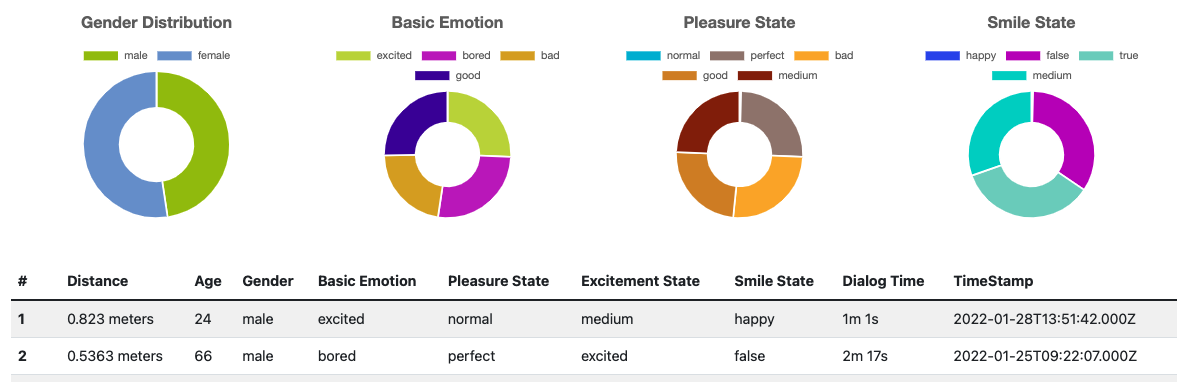
\includegraphics[width=\textwidth]{Figures/NodeChapter/adminDashboard2.png}
    \caption{Webansicht des Admin Dashboards Teil 2}
    \label{fig:admindashboard2}
    \centering
\end{figure}

Zusätzlich zur Darstellung der Konversationsverläufe haben wir uns entschieden, weitere interessante Informationen zu den zur Grunde
liegenden Gesprächen visuell hervorzuheben. Somit ist es möglich, sich einen schnellen Überblick
über die letzen Interaktionen mit Pepper zu gelangen.

(Abb. \ref{fig:admindashboard2}) Sprechen mehr männliche oder weibliche Personen
mit Pepper? Wie ist die Stimmung unserer Akteure und wie verhalten sie sich? Wird gelacht oder sind sie gelangweilt? Diese Informationen
können anhand der Donut-Diagrammen abgelesen und interpretiert werden. So hat man beispielsweise Auskunft darüber, ob ein neues
Update bei den Kunden und Anwendern gut ankommt, oder ob man nicht doch noch etwas ausbessern sollte. Zudem ist auf unseren
Anwendungsfall Hochschule bezogen, auch nachvollziehbar, wie die allgemeine Stimmung der Studenten und Interessierten ist.

Unterhalb den Diagrammen begint eine Tabelle, welche die ausgewerteten Datenreihen beinhaltet. Jede dieser Reihen
führt per Klick auf eine Detailansicht der jeweiligen Konversation und bietet somit einen genaueren Einblick in das geführte
Gespärch.

\begin{figure}[H]
    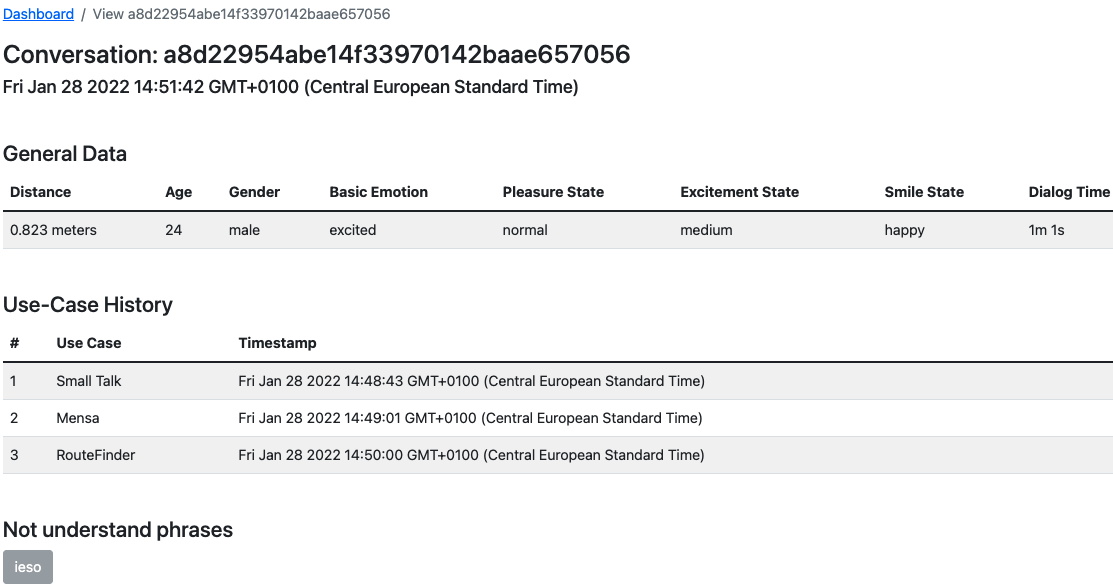
\includegraphics[width=\textwidth]{Figures/NodeChapter/webappdetail.png}
    \caption{Ansicht einer bestimmten Konversation}
    \label{fig:webappdetail}
    \centering
\end{figure}

(Abb. \ref{fig:webappdetail}) Jeder Konversation, die Pepper führt, wird eine Identifikationsnummer zugewisen. Dies ermöglicht
die dynamische Zuordnung von Inhalten zu einem bestimmten Gespräch. Somit ist eine neben der Einsicht in die allgemeinen Informationen
wie dem Alter und Geschlecht des Gespärchspartners möglich, auch Informationen über verwendete Anwendungsfälle und deren
chronologischer Reihenfolge zu erhalten. Auch Phrasen, welche Pepper nicht verstanden hat, sei es aufgrund von Akzenten oder
falscher Aussprache, werden der Konversation zugewiesen.

Dies alles ermöglicht es uns und dem Anwender der Software, mehr über seine Kunden und Anwender zu erfahren - oder auf die Hochschule
bezogen: Die Stimmung der Studenten, sowie des Personals und Interessierten kann somit erfasst werden.

\subsection{API}
\label{sec:nodechapter-api}
Die Kommunikation mit unserer Webanwendung verläuft nicht nur über das Web Interface, sondern über verschiedene Endpunkte,
auch Routes genannt. Über diese können je nach Grad der Authentifizierung verschiedene Inhalte gesendet und empfangen werden.

Um hier nicht zu viele Informationen aus den Bereichen der Endpunkte (\ref{sec:nodechapter-implementation-routes}) und Implementierung (\ref{sec:nodechapter-implementation}) vorweg zu nehmen,
wollen wir es bei der Erwähnug und Beschreibung der wichtigsten Endpunkte belassen.

\begin{itemize}
    \item /docker-hbv-kms-http/collector
    \item /docker-hbv-kms-http/getData
    \item /docker-hbv-kms-http/api/v1
\end{itemize}

Der Endpunkt ``collector'' dient der Speicherung verschiedener Informationen, welche Pepper an unserern Server über die
von ihm geführten Konversation sammelt (vgl. Abschnitt \ref{sec:api-save-data}). Dieser ist sowohl als GET, als auch über eine POST Anfrage erreichbar und nimmt
verschiedene Parameter entgegen. Bisher ist dieser Endpunk ohne Authentifizierung, das heißt, jeder der weiß, in welcher Form
die Daten übermittelt werden, kann Informationen in unsere Tabellen speichern.

Wir haben überlegt dies zu Umgehen, indem wir Pepper ein Token generieren lassen, welches nötig ist,
um die Daten zu speichern, jedoch würde dies das Problem nur verlagern, da unser gesamter Quellcode öffentlich einsehbar ist.
Dies kann nicht über Umgebungsvariablen umgangen werden, da dies in der Android Studio Umgebung zur Entwicklung von Android Anwendungen
nicht so zur Verfügung steht, wie wir es benötigen.

Der Endpunkt ``getData'' wird von dem Web Interface verwendet, um die Daten, welche sich in unserer Datenbank befindet abzurufen.
Dieser setzt voraus, dass der Benutzer als Admin angemeldet ist und ein gültiges JSON Web Token in seinem Cookie besitzt. (vgl. Abschnitt \ref{sec:routes-dashboard-query})

Der letzte Endpunkt in der Liste ``api/v1' ist die Schnittstelle über welche man extern auf Daten in der Datenbank zugreifen kann.
Hier ist es ebenfalls erforderlich, authentifiziert zu sein. Dafür muss ein Auth Token bei jeder Abfrage übermittelt werden,
welches mit dem in unserer Vebanwendung hinterlegten verglichen wird. Hierbei haben wir nich das Problem des öffentlichen
Einsehens in das Token, da wir dieses nicht über GitHub speichern. (vgl. Abschnitt \ref{sec:api-sql-query})

Es gibt natürlich noch viele weitere Endpunkte in unserer Webanwendung, wie zum Beispiel den zur Abfrage von Stunden- oder Mensaplänen.
Diese bekommen auch Parameter übergeben, woraufhin diese mit Hilfe verschiedener Methoden die gewünschten Informationen bereitstellen.
(vgl. Abschnitt \ref{sec:nodechapter-implementation-routes})

\subsection{Datenbank}
\label{sec:nodechapter-database}
Um die Informationen, welche unser Pepper während seiner Gespräche sammelt auch persistent speichern zu könenn,
haben wir uns dazu entschieden, eine MySQL Datenbank zu integrieren. Zunächst haben wir es als fortschrittlicher
gehalten, MongoDB zu verwenden, da dies eine JSON-Objekt basierte Speicherung von Daten ermöglicht und durch seine
skalierbare und einfache Integration in Expres und JavaScript vielfältige Möglichkeiten bietet.

MongoDB ist jedoch nicht auf dem Hochschulserver installiert und da wir durch verschiedene Kurse schon sehr gute Kenntnisse
und Erfahrungen mit MySQL gesammelt haben, war es dann doch nicht so schlimm, auf MongoDB zu verzichten.

Die von der Webanwendung verwendete Datenbank läuft in dem zuvor erwähnten Docker Kontainers des geteilten Benutzers.

Weitere Informationen und Spezifikationen sind der Tabelle im Abschnitt \ref{sec:nodechapter-versions} zu entnehmen.



% -------- -------- -------- -------- -------- -------- -------- -------- -------- -------- -------- 
% -------- -------- -------- -------- -------- -------- -------- -------- -------- -------- -------- 
% -------- -------- -------- -------- -------- -------- -------- -------- -------- -------- -------- 
% -------- -------- -------- -------- -------- -------- -------- -------- -------- -------- -------- 
% -------- -------- -------- -------- -------- -------- -------- -------- -------- -------- -------- 
% -------- -------- -------- -------- -------- -------- -------- -------- -------- -------- -------- 

\newpage
\section{Endpunkte und Responses der Webanwendung}
\label{sec:nodechapter-implementation-routes}
\lhead{Kapitel 6. \emph{Node - Express Webanwendung: Endpunkte und Responses}}
Unsere Webanwendung ist über viele Endpunkte ansprechbar.
Nachfolgend sind diese in zwei Gruppen Aufgeteilt.
Endpunkte, welche für das Admin Dashboard benötigt werden, sowie als Resultat eine HTML Seite rendern,
sind unter dem Abschnitt \ref{sec:routes} zu finden.
Alle weiteren Endpunkte, welche zumeist nur Daten entgegen nehmen oder Informationen in Form
von JSON zurück geben, sind in Abschnitt \ref{sec:api-routes} aufgelistet.

\subsection{Web Interface Endpunkte / Routes}
\label{sec:routes}
\dotfill
\subsubsection{Startseite}
\label{sec:routes-start}
\textbf{Beschreibung:} Liefert die Startseite der Webanwendung wieder. Auf dieser ist nur der Titel der Anwendung,
sowie einen Button, der zur Login Seite führt. (siehe \ref{sec:routes-login})

\textbf{Methode:} GET

\textbf{Endpunkt:} /docker-hbv-kms-http/

\textbf{Parameter:}
keine

\dotfill

\subsubsection{Dashboard}
\label{sec:routes-dashboard}
\textbf{Beschreibung:} Liefert einem angemeldetem Admin die Ansicht des Dashboards.
(vgl. Abb. \ref{fig:admindashboard1} und \ref{fig:admindashboard2})

\textbf{Methode:} GET

\textbf{Endpunkt:} /docker-hbv-kms-http/dashboard

\textbf{Parameter:}
keine

\dotfill

\subsubsection{Dashboard: Detailansicht}
\label{sec:routes-dashboard-detail}
\textbf{Beschreibung:} Dient der visuellen Übermittlung der Detailansicht einer Konversation (vgl. Abb. \ref{fig:webappdetail}).
Dies ist nur über den Browser erreichbar, sofern ein gültiges JSON Web Token im Cookie hinterlegt ist.

\textbf{Methode:} GET

\textbf{Endpunkt:} /docker-hbv-kms-http/dashboard/view

\textbf{Parameter:}
\begin{table}[H]
    % \caption{Hard- und Softwarespezifikationen}
    \label{table:/docker-hbv-kms-http/dashboard/view}
    \setlength{\tabcolsep}{3pt}
    \begin{tabular}{p{100pt}p{80pt}p{200pt}}
        \hline
        Param            & Typ    & Beschreibung                        \\                                                             \\
        \hline
        conversation\_id & String & ID der zu abzurufenden Konversation \\
        \hline
    \end{tabular}
\end{table}
\dotfill

\subsubsection{Dashboard: Datenabfrage}
\label{sec:routes-dashboard-query}
\textbf{Beschreibung:} Dieser Endpunkt dient der Abfrage von \textit{n} Datenreihen, welche auf dem Admin Dashboard
dargestellt werden. Dies wird für die Tabelle, sowie für die dortigen Visualisierungen verwendet.

\textbf{Methode:} GET

\textbf{Endpunkt:} /docker-hbv-kms-http/api/v1/getData

\textbf{Parameter:}
\begin{table}[H]
    \label{table:/docker-hbv-kms-http/api/v1/getData}
    \setlength{\tabcolsep}{3pt}
    \begin{tabular}{p{100pt}p{80pt}p{200pt}}
        \hline
        Param & Typ    & Beschreibung                        \\
        \hline
        n     & String & Anzahl der abzurufenden Datenreihen \\
        \hline
    \end{tabular}
\end{table}
\dotfill

\subsubsection{Login}
\label{sec:routes-login}
\textbf{Beschreibung:} Liefert bei einer GET Anfrage die Login Seite aus. Der POST Endpunkt wird
nach Abschicken des Login-Forumulars angesprochen, validiert den Login und leitet den Client bei
Erfolg an das Dashboard weiter. Gleichzeitig wird das JSON Web Token im Cookie des Clients hinterlegt.

\textbf{Methode:} GET, POST

\textbf{Endpunkt:} /docker-hbv-kms-http/dashboard/login

\textbf{Parameter GET:} keine

\textbf{Parameter POST:}
\begin{table}[H]
    \label{table:/docker-hbv-kms-http/login}
    \setlength{\tabcolsep}{3pt}
    \begin{tabular}{p{100pt}p{80pt}p{200pt}}
        \hline
        Param           & Typ    & Beschreibung \\                                                             \\
        \hline
        username\_input & String & Benutzername \\
        password\_input & String & Passwort     \\
        \hline
    \end{tabular}
\end{table}
\dotfill

\subsubsection{Logout}
\label{sec:routes-logout}
\textbf{Beschreibung:} Löscht das JSON Web Token aus dem Cookie des Benutzers und meldet ihn somit ab.
Anschließend wird nach /docker-hbv-kms-http/ weiter geleitet. (vgl. Abschnitt \ref{sec:routes-start})

\textbf{Methode:} GET

\textbf{Endpunkt:} /docker-hbv-kms-http/dashboard/logout

\textbf{Parameter:} keine

\dotfill






\subsection{API Endpunkte / Routes}
\label{sec:api-routes}
Alle Endpunkte, welche nicht über ein GUI angesprochen werden, sind mit ``api' in der URI hiterglegt. Anschließend
ist die Versionsnummer des Endpunktes anzugeben. Bisher gibt es nur die Version 1.

\subsubsection{Speicherung von Emotionsdaten}
\label{sec:api-saveEmotionData}
\textbf{Beschreibung:} Dieser Endpunkt dient der Speicherung verschiedener Daten, welche sich im Verlauf einer
Konversation mit Pepper ergeben.

\textbf{Methode:} GET

\textbf{Endpunkt:} /docker-hbv-kms-http/api/v1/saveEmotionData

\begin{table}[H]
    %\label{table:/docker-hbv-kms-http/api/v1/saveEmotionData}
    \setlength{\tabcolsep}{3pt}
    \begin{tabular}{p{100pt}p{80pt}p{200pt}}
        \hline
        Param             & Typ            & Beschreibung                                            \\
        \hline
        identifier        & String         & Identifikationsnummer der Konversation                  \\
        distance          & String / Float & [optional] Distanz zwischen Pepper und dem Sprecher     \\
        age               & String / Float & [optional] Alter des Sprechers                          \\
        gender            & String         & [optional] Geschlecht des Sprechers                     \\
        basic\_emotion    & String         & [optional] Generelle Stimmung des Sprechers             \\
        pleasure\_state   & String         & [optional] Motivation des Sprechers                     \\
        excitement\_state & String         & [optional] Begeisterung des Sprechers                   \\
        smile\_state      & String         & [optional] Einschätzung der Glücklichkeit des Sprechers \\
        dialog\_time      & String / Float & [optional] Zeit des Gespräches                          \\
        \hline
    \end{tabular}
\end{table}

\dotfill

\subsubsection{Speicherung des verwendeten Anwendungsfalles}
\label{sec:api-saveUseCaseData}
\textbf{Beschreibung:} Realisierung der Speicherung der in einer Konversation verwendeten Anwendungsfälle.

\textbf{Methode:} GET

\textbf{Endpunkt:} /docker-hbv-kms-http/api/v1/saveUseCaseData

\begin{table}[H]
    \label{table:/docker-hbv-kms-http/api/v1/saveUseCaseData}
    \setlength{\tabcolsep}{3pt}
    \begin{tabular}{p{100pt}p{80pt}p{200pt}}
        \hline
        Param      & Typ    & Beschreibung                           \\
        \hline
        identifier & String & Identifikationsnummer der Konversation \\
        use\_case  & String & Name des Use-Cases                     \\
        \hline
    \end{tabular}
\end{table}

\dotfill

\subsubsection{Speicherung von nicht verstandenen Phrasen}
\label{sec:api-saveNotUnderstandPhrases}
\textbf{Beschreibung:} Realisierung der Speicherung der von Pepper nicht verstandenen Wörter und Phrasen.

\textbf{Methode:} GET

\textbf{Endpunkt:} /docker-hbv-kms-http/api/v1/saveNotUnderstandPhrases

\begin{table}[H]
    \label{table:/docker-hbv-kms-http/api/v1/saveNotUnderstandPhrases}
    \setlength{\tabcolsep}{3pt}
    \begin{tabular}{p{100pt}p{80pt}p{200pt}}
        \hline
        Param      & Typ    & Beschreibung                           \\
        \hline
        identifier & String & Identifikationsnummer der Konversation \\
        phrase     & String & Nicht verstandene Phrase               \\
        \hline
    \end{tabular}
\end{table}

\dotfill

\subsubsection{Speicherung von zusätzlichen Daten}
\label{sec:api-saveAttributeData}
\textbf{Beschreibung:} Dieser Endpunkt ermöglicht die Speicherung von weiteren, variablen und nicht
vordefinierten Informationen.

\textbf{Methode:} POST

\textbf{Endpunkt:} /docker-hbv-kms-http/api/v1/saveAttributeData

\begin{table}[H]
    \label{table:/docker-hbv-kms-http/api/v1/saveAttributeData}
    \setlength{\tabcolsep}{3pt}
    \begin{tabular}{p{100pt}p{80pt}p{200pt}}
        \hline
        Param      & Typ           & Beschreibung                           \\
        \hline
        identifier & String        & Identifikationsnummer der Konversation \\
        data       & String / JSON & variable Daten der Konversation        \\
        \hline
    \end{tabular}
\end{table}
\dotfill



\subsubsection{Abfrage von Daten aus der DB mittels SQL Query String}
\label{sec:api-sql-query}
\textbf{Beschreibung:} Endpunkt zur Interaktion mit der Datenbank. Ein API-Token wird benötigt. SQL Befehle können
übermittelt werden. Aus sicherheitsgründen werden Anfragen, welche folgende Wörter beinhalen, abgelehnt:
``drop'', ``delete'', ``show'', ``users'', ``insert'', ``into'', ``create''. Bei erfolgreicher
Abfrage wird das Ergebnis des SQL-Statements als JSON zurückgeliefert.

\textbf{Methode:} POST

\textbf{Endpunkt:} /docker-hbv-kms-http/api/v1/sql

\textbf{Parameter:}
\begin{table}[H]
    \label{table:/docker-hbv-kms-http/api/v1/sql}
    \setlength{\tabcolsep}{3pt}
    \begin{tabular}{p{100pt}p{80pt}p{200pt}}
        \hline
        Param      & Typ    & Beschreibung               \\
        \hline
        auth\_key  & String & API-Token                  \\
        subject    & String & [optional] Art der Abfrage \\
        sql\_query & String & Auszuführender SQL Befehl  \\
        \hline
    \end{tabular}
\end{table}
\dotfill

\subsubsection{Abfrage des Stundenplans}
\label{sec:api-timetable}
\textbf{Beschreibung:} Dient der Abfrage von Stundenplänen eines bestimmten Studiengangs.
Bei erfolgreicher Abfrage wird ein JSON Objekt, oder einen HTML String zurückgegeben.

\textbf{Methode:} GET

\textbf{Endpunkt:} /docker-hbv-kms-http/api/v1/timetable

\textbf{Parameter:}
\begin{table}[H]
    \label{table:/docker-hbv-kms-http/api/v1/timetable}
    \setlength{\tabcolsep}{3pt}
    \begin{tabular}{p{100pt}p{80pt}p{200pt}}
        \hline
        Param    & Typ          & Beschreibung                                        \\
        \hline
        course   & String       & Studiengang (Kürzel wie: ``WI'', ``BWL'' etc.)      \\
        kw       & String / Int & [optional] Kalenderwoche                            \\
        semester & String / Int & [optional] Semester                                 \\
        htmlOnly & Boolean      & [optional] HTML oder JSON Response (Default: false) \\
        \hline
    \end{tabular}
\end{table}
\dotfill


\subsubsection{Abfrage des Mensaplans als JSON}
\label{sec:api-mensa-json}
\textbf{Beschreibung:} Liefert den Mensaplan für die aktuelle Woche als JSON Objekt zurück.
\textbf{Methode:} GET

\textbf{Endpunkt:} /docker-hbv-kms-http/api/v1/mensadata

\textbf{Parameter:} keine

\dotfill

\subsubsection{Abfrage des Mensaplans als Bild}
\label{sec:api-mensa-img}
\textbf{Beschreibung:} Liefert den Mensaplan fur die aktuelle Woche als Bild zurück.

\textbf{Methode:} GET

\textbf{Endpunkt:} /docker-hbv-kms-http/api/v1/mensadata/img

\textbf{Parameter:} keine

\dotfill

\subsubsection{File Server}
\label{sec:api-fileserver}
\textbf{Beschreibung:} Dieser Endpunkt wird verwendet, Skripte und Stylesheets dynamisch aus dem ``static'' Verzeichnis
abzurufen.

\textbf{Methode:} GET

\textbf{Endpunkt:} /docker-hbv-kms-http/fileserver

\textbf{Parameter:}
\begin{table}[H]
    \label{table:/docker-hbv-kms-http/fileserver}
    \setlength{\tabcolsep}{3pt}
    \begin{tabular}{p{100pt}p{80pt}p{200pt}}
        \hline
        Param & Typ    & Beschreibung                 \\
        \hline
        name  & String & Name der angeforderten Datei \\
        \hline
    \end{tabular}
\end{table}
\dotfill


\subsubsection{Abfrage des Kurspreises einer Kryptowährung}
\label{sec:api-crypto}
\textbf{Beschreibung:} Dieser Endpunkt kann einem den Kurspreis und weitere relevante Informationen zu einem
Kryptowährungs-Handelspaar zurückliefern.

\textbf{Methode:} GET

\textbf{Endpunkt:} /docker-hbv-kms-http/api/v1/crypto

\textbf{Parameter:}
\begin{table}[H]
    \label{table:/docker-hbv-kms-http/api/v1/crypto}
    \setlength{\tabcolsep}{3pt}
    \begin{tabular}{p{100pt}p{80pt}p{200pt}}
        \hline
        Param    & Typ    & Beschreibung                                  \\
        \hline
        subject  & String & Anforderung (nur ``price'' ist implementiert) \\
        ksymbolw & String & Symbol (Bsp.: ``BTC-USDT'')                   \\
        \hline
    \end{tabular}
\end{table}
\dotfill

\subsubsection{Abfrage der IP-Adresse des Clients}
\label{sec:api-client-ip}
\textbf{Beschreibung:} Liefert die IP Adresse des Clients zurück.

\textbf{Methode:} GET

\textbf{Endpunkt:} /docker-hbv-kms-http/api/v1/ip

\textbf{Parameter:} keine

\dotfill


\subsection{Responses und Status Codes}
\label{sec:nodechapter-implementation-responses}
Alle An- und Abfragen an unsere Webanwendung liefern verschiedene Antworten / Responses zurück. In der nachfolgenden Tabelle
sind die Geläufigsten aufgelistet. Da gewisse Error-Handling Mechanismen automatisch eine entsprecheende Antwort liefern,
kann es zu abweichenden Beschreibungen und weiteren Status Codes kommen.
\begin{table}[H]
    \label{table:responsecodes}
    \setlength{\tabcolsep}{3pt}
    \begin{tabular}{p{100pt}p{280pt}}
        \hline
        Status Code & Bedeutung                          \\
        \hline
        200         & OK                                 \\
        401         & ungültige Parameter                \\
        404         & Datei oder Endpunkt nicht gefunden \\
        500         & Interner Server Fehler             \\
        \hline
    \end{tabular}
\end{table}

% -------- -------- -------- -------- -------- -------- -------- -------- -------- -------- -------- 
% -------- -------- -------- -------- -------- -------- -------- -------- -------- -------- -------- 
% -------- -------- -------- -------- -------- -------- -------- -------- -------- -------- -------- 
% -------- -------- -------- -------- -------- -------- -------- -------- -------- -------- -------- 
% -------- -------- -------- -------- -------- -------- -------- -------- -------- -------- -------- 
% -------- -------- -------- -------- -------- -------- -------- -------- -------- -------- -------- 

\newpage
\section{Implementierung}
\label{sec:nodechapter-implementation}
\lhead{Kapitel 6. \emph{Node - Express Webanwendung: Implementierung}}
Bei unserer Web App handelt es sich um eine Anwendung, welche mit dem Framework Express für die Laufzeitumgebung
Node entwickelt wurde. Express zeichnet sich durch die simple Konfiguration, sowie einfache Implementierung
verschiedenster Funktionalitäten aus. Express wird meist für Backendanwendungen verwendet, wir benutzen es jedoch auch,
um serverseitiges Rendering zu realisieren. Dies bedeutet, dass Ansichten (Views), welche an den Client ausgeliefert werden,
zuvor auf dem Server gerendert worden sind.

Von außen ist unsere Anwendung über die URL
\href{https://informatik.hs-bremerhaven.de/docker-hbv-kms-http}{https://informatik.hs-bremerhaven.de/docker-hbv-kms-http}
erreichbar. Sollte sie lokal ausgeführt werden, muss die Domain auf Localhost geändert werden - hier ist dann auch die Angabe
des Ports nötig. (mehr dazu in Abschnitt \ref{sec:nodechapter-implementation-config})


Unsere Anwendung besitzt jedoch nicht all zu viele Views, bis auf das zuvor gezeigte Admin Dashboard (vgl. Abschnitt \ref{sec:routes-dashboard}), sowie
die Detailansicht der einzelnen Daten der Konversationen (vgl. Abschnitt \ref{sec:routes-dashboard-detail}). Darüber hinaus gibt es nur
die Startseite (vgl. ABschnitt \ref{sec:routes-start}) und die Login-View. Diese Login-View ist über den Endpunkt ``/docker-hbv-kms-http/login'' (vgl. Abschnitt \ref{sec:routes-login}) erreichbar und beinhaltet nur ein Formular zur Eingabe des
Benutzernamens, sowie des dazugehörigen Passwortes.


Abbildung \ref{fig:webhierarchie} zeigt den Inhalt des Root-Verzeichnisses unserer Webanwendung.
Im Folgenden wird auf die einzelnen Inhalte eingegangen. \\

\begin{figure}[H]
    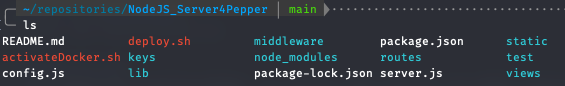
\includegraphics[width=\textwidth]{Figures/NodeChapter/ServerFileStructure.png}
    \caption{Hierarchie des Stammverzeichnisses der Webanwendung}
    \label{fig:webhierarchie}
    \centering
\end{figure}

\subsubsection*{server.js}
Der Einstiegspunkt unserer Webanwendung ist das Skript ``server.js''. Dieses beinhaltet die Einbindung aller
benötigten Dateien und Skripte, sowie die Anwendung der in den Konfigurationsdateien festgelegten Einstellungen
(mehr dazu in Abschnitt \ref{sec:nodechapter-implementation-config}).

\subsubsection*{node\_modules, package-lock.json und package.json}
Da wir Node als Laufzeitumgebung gewählt haben, ist es uns möglich den Node Package Manager (npm) zur Installation
verschiedener Module anzuwenden. Alle installierten Module sind in dem Verzeichnis ``node\_modules'' zu finden.
Deren Spezifikationen sind in den Konfigurationsdateien ``package.json'', sowie ``package-lock.json'' festgehalten.
package-lock.json ist eine automatisch generierte Datei, welche Node verwendet um Dependencies und Versionen festzuhalten.
Aufgrund dieser Konfigurationsdateien ist es nicht nötig, alle im Verzeichnis ``node\_modules' befindlichen Erweiterungen
in das jeweilige GitHub Repository zu laden, denn diese können, nach einer neuen Initialisierung über den Befehl ``npm init''
anhand der Definitionen in package-lock.json, automatisch nachinstalliert werden.

\subsubsection*{views}
In diesem Verzeichnis befinden sich Templates der Seiten, welche vom Server gerendert und an den Client ausgeliefert werden.

\subsubsection*{routes}
Der Ordner ``routes'' beinhaltet die verschiedene Skripte, welche die unterschiedlichen Endpunkte unserer Webanwendung definieren.
Innerhalb dieser Skritpe werden auch die Ansichten aus dem ``views''-Verzeichnis gerendert und an den Client geschickt. Hier sind alle
in Abschnitt \ref{sec:nodechapter-implementation-routes} behandelten Endpunkte definiert.

\subsubsection*{static}
Hier finden sich statische Dateien, hierzu gehören Bilder und unabhängige Skripte, sowie Stylesheets.

\subsubsection*{middleware}
Bei Middlewares handelt es sich um Skripte, welche Abläufe beinhalten, die zwischen anderen Prozessen statt finden.
Hierzu gehört bei uns die Authentifizierung von Nutzern, indem das sich dort befindliche Skript ``auth.js'' eingebunden wird,
während ein Nutzer einen beschränkten Endpunkt anspricht. Dies sorgt dafür, dass nur ausgewählte Benutzer bestimmte Endpunkte
erfolreich ansprechen können. Alle anderen bekommen die Mitteilung, dass sie nicht die nötigen Berechtigunen besitzen.

\subsubsection*{lib}
Im Ordner lib (aka Libraries) befinden sich alle von uns für die Webanwendung verwendeten Skripte, für welche wir keine genaue
Unterkategorie finden konnten. Hierbei handelt es sich um Skripte, welche Anfragen (Requests) synchron und asynchron durchführen können,
sowie Funktionen zur Generierung und Validierung von Passwörtern und deren Hash.

\subsubsection*{keys}
Da wir beschränkte Endpunkte haben und unsere Authentifizierung mittels JSON Web Token im Cookie des Clients realisiert ist,
muss unsere Anwendung dieses Token auch auf Richtigkeit überprüfen können. Daher haben wir uns dazu entschieden ein Schlüsselpaar
zu generieren, welches für die Ver-und Entschlüsselung der JSON Web Token verwendet wird.

\subsubsection*{Sonstige Dateien}
Im Hauptverzeichnis befinden sich weitere Dateien, wie die README.md, welche eine Quick-Start Anleitung bietet, die in
dem \href{https://github.com/ProjectPepperHSB/NodeJS_Server4Pepper}{Repository} der Webanwendung dargestellt ist.

Des weiteren befindet sich ein Skript zum Aktivieren des Docker-Kontainers und ein Deploy-Skript, welches
für die Aktivierung des Dockers, das Übertragen der Daten in das entsprechende Verzeichnis, sowie für den Start der
Webanwendung sorgt.

Im Repository ist auch die Datei ``.example.env'' zu finden, welche ein Beispiel dafür bietet, wie die ``.env'' Datei
aussehen muss. Diese .env Datei legt Umgebungsvariablen fest, sowie beinhaltet es sensible Daten, wie
die Informationen zum Login in die Datenbank, sowie den API-Key zur Nutzung der API über externe Programme / Skripte
(vgl. Abschnitt \ref{sec:api-sql-query}).



\subsection{Error-Handling}
\label{sec:nodechapter-error-handling}


\subsection{Konfiguration}
\label{sec:nodechapter-implementation-config}

% .env 
%config.js 
% port bei lokalhost
% Admin user wird automatisch angelegt
% Datenschutz und Datensicherheit 



\subsection{Versionen und Spezifikationen}
\label{sec:nodechapter-versions}
% Unsere Webanwendung basiert auf NodeJS und JavaScript. NodeJS ist eine Laufzeitumgebung, welche JavaScript außerhalb des Browsers
% ausführen kann und somit wichtige Prozesse auf dem Server anstatt beim Client ausführen kann. NodeJS hat einen eigenen Paketmanager,
% npm (Node Package Manager), mit welchem sich vielfältige Libraries und Frameworks installieren und ausführen lassen.

% ... wir nutzen das Modul Express, welches es uns ermöglicht, ohne großen Aufwand, eine vollig anpassbare Webanwendung zu erstellen.

MySQL: Ver 15.1 Distrib 10.6.5-MariaDB, for debian-linux-gnu
\newpage
\section{Installation}
\label{sec:nodechapter-installation}
\lhead{Kapitel 6. \emph{Node - Express Webanwendung: Installation}}
erst dies, dann dass und ananas
ggf. muss das Deploy Skript angepasst werden
\newpage
\section{Möglichkeiten der Erweiterung}
\lhead{Kapitel 6. \emph{Node - Express Webanwendung: mögl. der Erweiterung}}
